\section{Compilers}
A compiler is a computer program that translates computer code written in one programming language (the source language) into another language (the target language). Is during this translation process where the compiler validates the syntax and the semantics of the program, if any error is detected in the process the compiler raises an exception (understand as a compiler event that avoids the compiler to continue its execution).

\subsection{Internal Structure}
In order to decompose the internal structure of a compiler they have been split in to the most common task they do \reffig{compiler-stages}, of course this doesn’t mean that there are compilers with more or less stages, but at the end everything can be group into any of the groups that we will explain:

\begin{figure}[hb]
  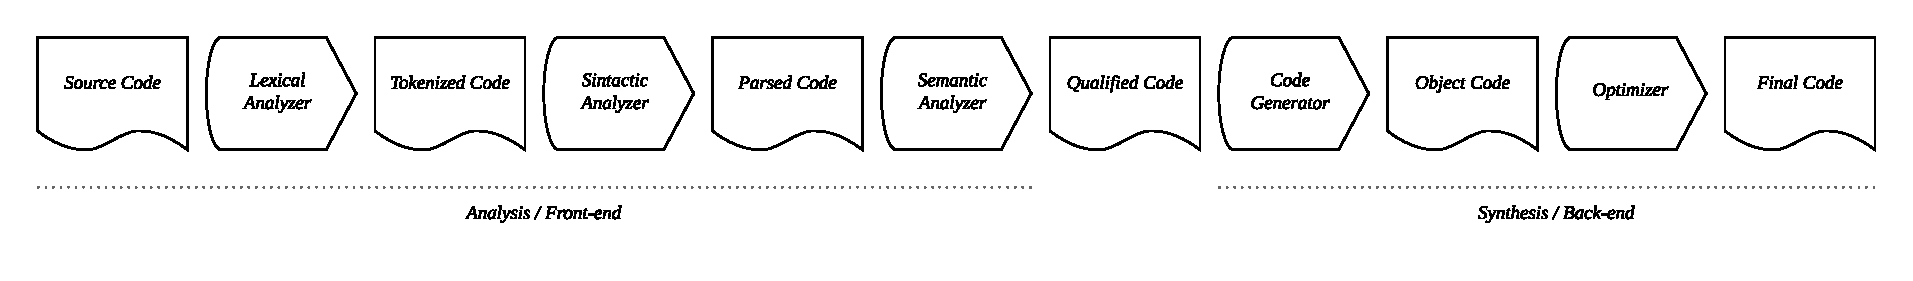
\includegraphics[width=50mm,scale=0.5]{compiler-stages}
  \caption[Compiler stages]{Compiler stages.}
  \labfig{compiler-stages}
\end{figure}

\subsubsection{Lexycal Analyzer}
The lexical analyzer task is to get the input and split it in to tokens \sidecite{lexical-analysis}, which are build from lexemes. If the compiler cannot find a valid token for some lexemes in the source code will generate an error, as the input cannot be recognized.

\subsubsection{Syntactic Analyzer}
The syntactic analyzer takes the tokens generated during the lexical analysis and parses them in such a way that try’s to group tokens so the conform to the language grammar rules. During this stage if there is any error while trying to group the tokens then the compiler will rise an error as the input cannot be parsed.

\subsubsection{Semantic Analyzer}
The semantic analyzer has two main tasks, usually. First it validates that the source code semantics are correct, for example 4 + “aaa” would not make sense. And the second task is to transform the Abstract Syntax Tree in to a type-checked and annotated AST. Usually that means relate the invocations and variables to its definition, very useful for type-checking.

\subsubsection{Code Generator}
The task of the code generator as its name indicates is to generate the target code, it can be byte code, machine code or even another high-language code.

\subsubsection{Code Optimizer}
The code optimizer is the last step before the final target code is generated, it rewrites the code that the code generator produced without changing the semantics of the program, its aim is just to make code faster. At \sidecite{compiler-optimizations} you can see an example of some optimizations that can be done at compile time to make your code faster.

\subsection{Conventional Compilers}
Conventional compiler are a big monolith where each stage \reffig{compiler-stages} is executed automatically after the previous stage, if the compiler has eight steps you need to execute them all at once. This approach have been the “old-fashion” but it presents some drawbacks:
\begin{itemize}
	\item A poor IDE \sidecite{ide} integration. IDE’s need to perform incremental compilations in matter of nanoseconds so the user doesn’t feel lag when typing the program. With conventional compilers as you need to go through all the compilation process at once they where very slow and companies like Microsoft need to develop different compilers, one for the IDE and another for the final compilation of the program itself. This lead to several problems like that if a feature gets implemented in the final compilation compiler but not in the IDE one the IDE would not support the feature meanwhile the language would.
	\item Difficult to debug. As the conventional compilers where a blackbox the only way to test intermediate stages was by throwing an input and waiting the the feature you wanted to test was thrown for that input.
\end{itemize}

\subsection{Modern Compilers}
After the problems Microsoft had with the C\# compiler they decide to rewrite the whole compiler and introduce a concept called “compiler as an API” with Roslyn \sidecite{dotNet}. This concept has been perfectly accepted and solved many problems. In this concept each stage has an input and an output that can be accessed from outside the compiler and stages can be executed independently on demand. This means that for example if an IDE just want to execute the Lexer the Parser and the Semantic analysis it can. That translates in to speed for the user.

Also the second problem is solved as testing individual parts of the compiler is much more easy than the hole compiler at once.
